%  sample eprint article in LaTeX           --- M. Peskin, 9/7/00
%  modified for LHCP2017, lhcp2017@sjtu.edu.cn
%  This file is part of a tar file, which can be downloaded from the LHCP2017 indico site. 
%   https://indico.cern.ch/event/517784/overview 
% 


\documentclass[10pt]{article}
\usepackage{graphicx}



%%%%%%%%%%%%%%%%%%%%%%%%%%%%%%%%%%%%%%%%%%%%%%%%%%%%%%%%%%%%%%%%%%%%%%%%%%%%
%   document style macros
%%%%%%%%%%%%%%%%%%%%%%%%%%%%%%%%%%%%%%%%%%%%%%%%%%%%%%%%%%%%%%%%%%%%%%%%%%%%
\def\Title#1{\begin{center} {\Large #1 } \end{center}}
\def\Author#1{\begin{center}{ \sc #1} \end{center}}
\def\Address#1{\begin{center}{ \it #1} \end{center}}
\def\andauth{\begin{center}{and} \end{center}}
\def\submit#1{\begin{center}Submitted to {\sl #1} \end{center}}
\newcommand\pubblock{\rightline{\begin{tabular}{l} Proceedings of the Fifth Annual LHCP\\ 
         \pubdate  \end{tabular}}}

\newenvironment{Abstract}{\begin{quotation} \begin{center} 
             \large ABSTRACT \end{center}\bigskip 
      \begin{center}\begin{large}}{\end{large}\end{center} \end{quotation}}

\newenvironment{Presented}{\begin{quotation} \begin{center} 
             PRESENTED AT\end{center}\bigskip 
      \begin{center}\begin{large}}{\end{large}\end{center} \end{quotation}}

\def\Acknowledgements{\bigskip  \bigskip \begin{center} \begin{large}
             \bf ACKNOWLEDGEMENTS \end{large}\end{center}}
%%%%%%%%%%%%%%%%%%%%%%%%%%%%%%%%%%%%%%%%%%%%%%%%%%%%%%%%%%%%%%%%%%%%%%%%%%%%
%  personal abbreviations and macros
%    the following package contains macros used in this document:
\input econfmacros.tex
%%%%%%%%%%%%%%%%%%%%%%%%%%%%%%%%%%%%%%%%%%%%%%%%%%%%%%%%%%%%%%%%%%%%%%%%%%%

\textwidth=6.5in  \textheight=8.75in
\hoffset=-.85in
\voffset=-0.6in

%%  DO NOT CHANGE anything above.

% include packages you will need
\usepackage{color}

%%%%%%%%%%%%%%%%%%%%%%%%%%%%%%%%%%%%%%%%%%%%%%%%%%%%%%%%%%%%%%%%%%%%
% basic data for the eprint:
%%%%%%%%%%%%%%%%%%%%%%%%%%%%%%%%%%%%%%%%%%%%%%%%%%%%%%%%%%%%%%%%%%%%

% Instruction:
% Please change each of the following fields:
%

%% date
\newcommand\pubdate{\today}

%%  Affiliation
\def\affiliation{
On behalf of the XYZ Experiment, \\
Department of Physics \\
University of Wisconsin -- Madison, Madison, USA}

\begin{document}

% large size for the first page
\large
\begin{titlepage}
\pubblock


%% Change the title, name, abstract
%% Title 
\vfill
\Title{  THE TITLE OF YOUR PROCEEDINGS  }
\vfill

%  if you need to add the support use this, fill the \support definition above. 
%   \Author{ FIRSTNAME LASTNAME \support }
\Author{ Kenneth Long }
\Address{\affiliation}
\vfill
\begin{Abstract}

We summarize recent results from the CMS experiment on the simultaneous 
production of multiple vector bosons in proton-proton collisions at the 
CERN LHC. Unfolded differential distributions are presented at 8 TeV for
$WZ$ production and at 13 TeV for ZZ production.
Cross section measurements are presented for ZZ, $Z(\nu\nu)\gamma$ and 
$WZ$ production at 8 and 13 TeV. Limits on anomalous triple gauge couplings
are presented for WV ($V = W,Z \rightarrow q\bar{q}$ at 8 and 13 TeV.


\end{Abstract}
\vfill

% DO NOT CHANGE 
\begin{Presented}
The Fifth Annual Conference\\
 on Large Hadron Collider Physics \\
Shanghai Jiao Tong University, Shanghai, China\\ 
May 15-20, 2017
\end{Presented}
\vfill
\end{titlepage}
\def\thefootnote{\fnsymbol{footnote}}
\setcounter{footnote}{0}
%

% normal size for the rest
\normalsize 

%% Your paper should be entered below. 

\section{Introduction}

HERE IS YOUR INTRODUCTION, REPLACE THE TEXT

The program will be devoted to a review of the latest experimental and theoretical results on hadron collider physics and a discussion on the outlook for the coming years. The conference intends to provide a lively discussion between experimenters and theorists on topics such as the Standard Model Physics and Beyond, the Higgs Boson, Supersymmetry and Heavy Ion Physics and planning for the high luminosity upgrades.

\section{Observations}

REPLACE THE TEXT, FIGURE and TABLE.

%%%%%%%%%%%%%%%%%%%%%%%%%%%%%%%%%%%%%%%%%%%%%%%%%%%%%%%%%%%%%%%%%%%%%%%%%
%%
%%   use this format to include an .eps figure into your paper
%%
\begin{figure}[htb]
\centering
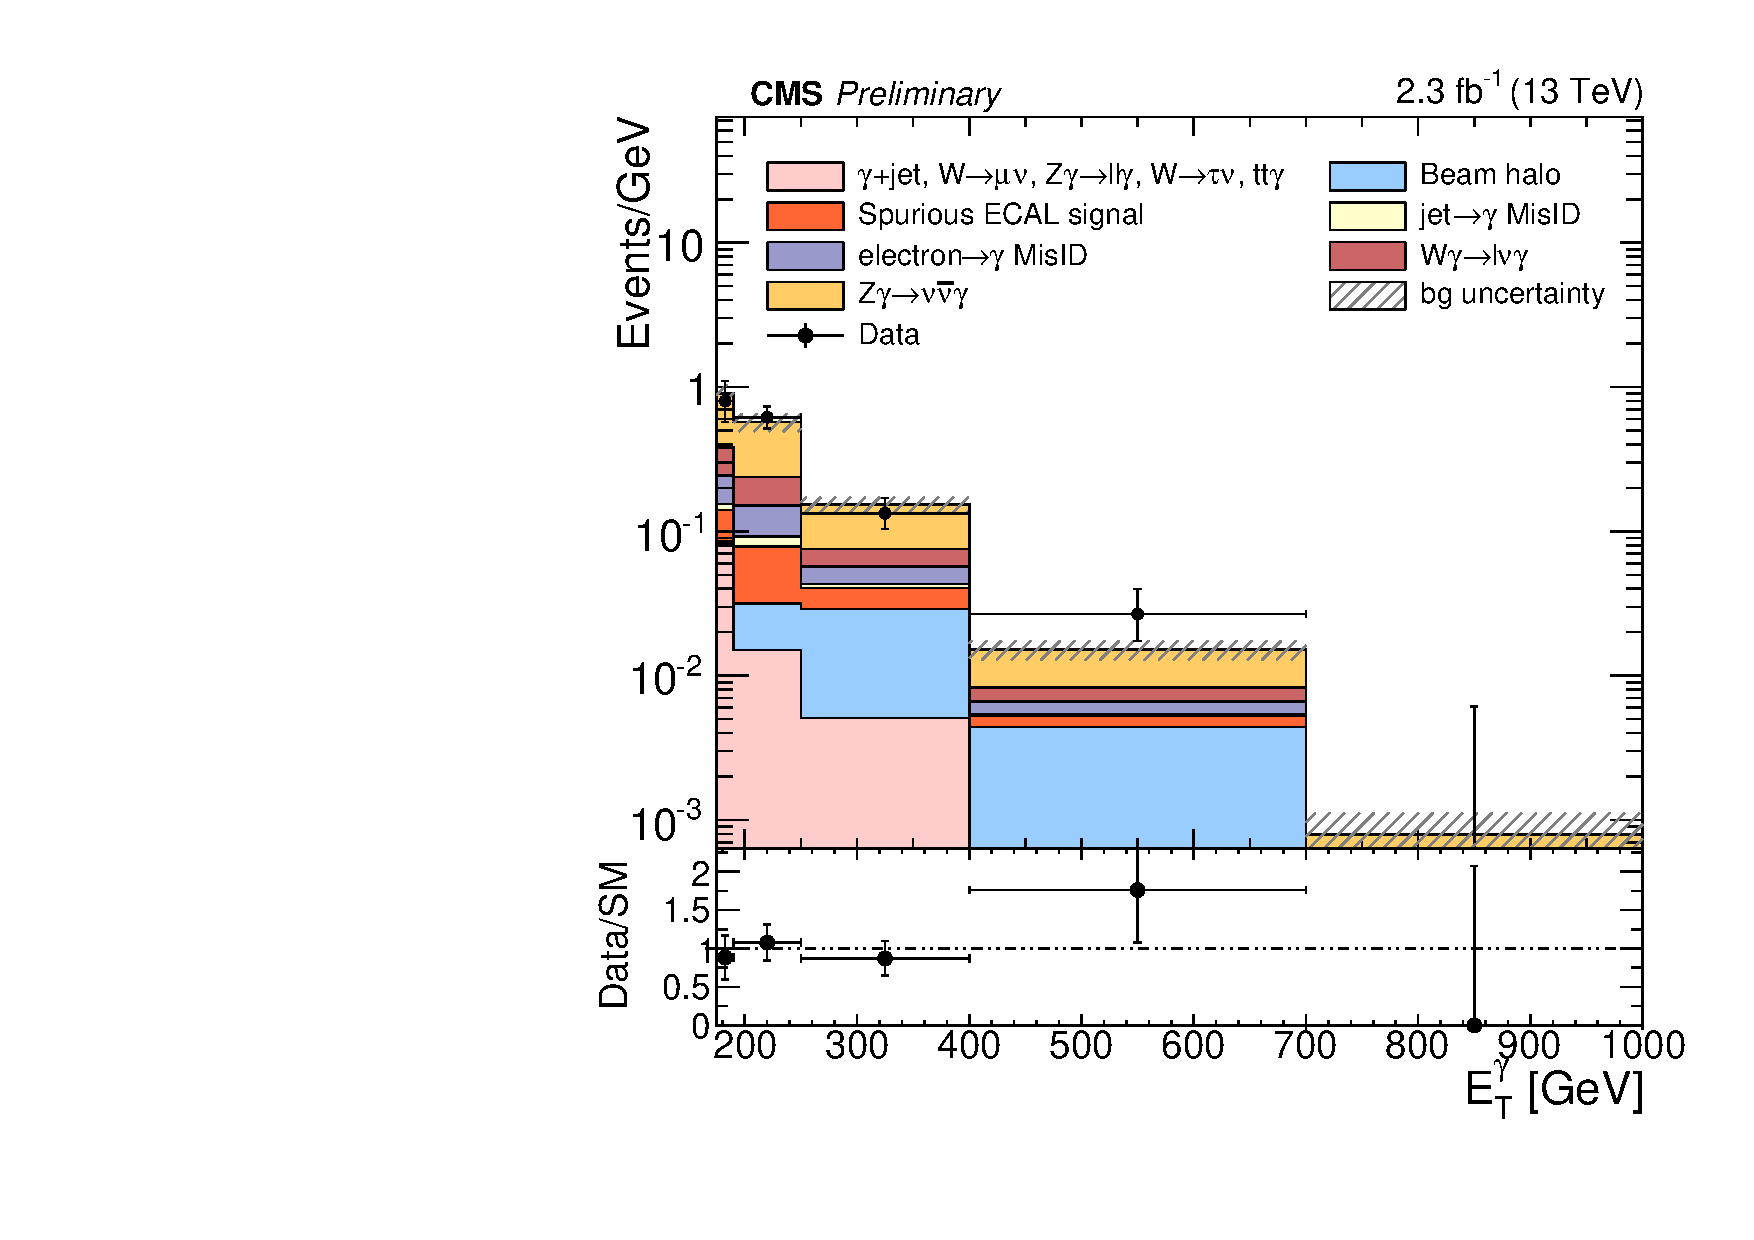
\includegraphics[height=2in]{figures/MonoPhoto_ETmiss.pdf}
\caption{ Place the caption here}
\label{fig:figure1}
\end{figure}
%%%%%%%%%%%%%%%%%%%%%%%%%%%%%%%%%%%%%%%%%%%%%%%%%%%%%%%%%%%%%%%%%%%%%%%%%%%
%
%%%%%%%%%%%%%%%%%%%%%%%%%%%%%%%%%%%%%%%%%%%%%%%%%%%%%%%%%%%%%%%%%%%%%%%%%
%%
%%   use this format to include a LaTeX table  into your paper
%%
%\begin{table}[t]
%\begin{center}
%\begin{tabular}{l|ccc}  
%Patient &  Initial level($\mu$g/cc) &  w. Magnet &  
%w. Magnet and Sound \\ \hline
% Guglielmo B.  &   0.12     &     0.10      &     0.001  \\
% Ferrando di N. &  0.15     &     0.11      &  $< 0.0005$ \\ \hline
%\end{tabular}
%\caption{ place the caption here }
%\label{tab:table1}
%\end{center}
%\end{table}
%%%%%%%%%%%%%%%%%%%%%%%%%%%%%%%%%%%%%%%%%%%%%%%%%%%%%%%%%%%%%%%%%%%%%%%%%%%

%and Table \ref{tab:table1}. 

\section{Differential and Inclusive Cross Section Measurements}

\subsection{$Z(\nu\nu)\gamma$ Production}
See Figure \ref{fig:figure1}
\cite{CMS-PAS-SMP-16-004}
\subsection{$W^{\pm}Z$ Production at 8 and 13 TeV}
\cite{Khachatryan:2016tgp}
\cite{Khachatryan:2016poo}
\subsection{$ZZ$ Production}
\cite{CMS:2017ruh}
\cite{CMS-PAS-SMP-16-019}

\section{Limits on Anomalous Gauge Couplings}

\subsection{Limits from $WV$ Production With Semil-leptonic Decays}

\subsection{Limits from Diboson States with Fully Leptonic Decays}


\section{Conclusions}

...... \cite{CMS:2016djf} \cite{Cascioli:2014yka} 

\bibliographystyle{JHEP}
\bibliography{bibliography}
\end{document}
